\documentclass[../main.tex]{report}
	
\begin{document}
    \label{sec:odd_prob}
\subsubsection{Ensembles probabilistes impairs}
Bien que ces ensembles aléatoires suivent la distribution de $\pi(x)$, il manque une propriété importante des nombres premiers: à l'exception de $2$, tous les nombres premiers sont impairs.
Nous allons alors modifier l'algorithme mentionné précedemment afin de générer des ensembles ayant cette propriété. 
%Soit $O_n := E_n \cap 2 \mathbb{N} +1$ l'ensemble des entiers impairs inférieurs à $n$. 
Soient alors les ensembles $R'_{k} \subset \{2\mathbb{N}+1 \cup \{2\}\}$ tels que $\forall~i \in \{2\mathbb{N}+1 \cup \{2\}\}$, le probabililité que $i$ soit dans l'ensemble $R'_{k}$ soit:

\[
P(i \in R'_{k}) = 
\left\{ 
    \begin{array}{cl}
         0 & \mbox{si}~i = 1 \\
         1 & \mbox{si}~ 2 \leq i < 9 \\
         \frac{2}{\log n} & \mbox{si}~i \geq 9
    \end{array}
\right.
\]

Le fait que $P(i \in R'_{k}) = 1$ pour les entiers impairs inferieurs à 9 découle du au fait que $2/\log(n) > 1$ pour ces entiers.

Ces ensembles débutent tous avec les mêmes éléments: $ (2,3,5,7,...) $, mais contienent ensuite des éléments choisis aléatoirement à partir du 5\up{e} terme. 
Pour tout $n \in 2\mathbb{N}+1, n\geq 5$, la fonction cette les fonctions $\sigma_{R'_k}$ sont donc des variables aléatoires. Pour simplfier l'écriture dans les sommations ci-dessous, nous posons, pour tout $n \in 2\mathbb{N} + 1, m:= \lfloor 2/n \rfloor$, de sorte que $2m-1$ soit bien le plus grand entier impair inférieur à $n$.
Notons $\sigma_{R'}$ la fonction mesurant l'esperance des fonctions $\sigma_{R'_k}$ en fonction de $n$.
\[
\sigma_{R'}(n)
= 4 + \frac{2}{\log 9} + \frac{2}{\log 11} + ...
= 4 + \sum_{i=5}^m \frac{2}{\log (2i-1)}
\]

%Nous allons maintenant définir, pour un certain $n \in 2\mathbb{N}-1, n \geq 5$, la fonction $g(n)$ comme un fonction en escalier de pas constant = 2:
%\[
%Li(n) = 
%\int_2^n \frac{dt}{\log t} = 
%\int_2^9 \frac{dt}{\log t} + \int_9^n \frac{dt}{\log t} \leq 
%Li(9) + \frac{2}{\log 9} + \frac{2}{\log 11} + ... = 
%Li(9) + \sum_{k=5}^{\lfloor\frac{n}{2}\rfloor} \frac{2}{\log(2k-1)} =: g(n)
%\]
%
%On a alors $g(n) = E[\sigma(n)] + Li(9) - 4$ 
%L'erreur entre Li et $g$ est bornée:
%\[
	%\begin{aligned}
%{\left| g(n) - Li(n) \right|} &= \left| Li(9) + \sum_{k=5}^{\lfloor\frac{n}{2}\rfloor} \frac{2}{2k-1} 
		%- (Li(9) + \int_9^n \frac{dt}{\log t} ) \right| \\ 
%&=\left| \sum_{k=5}^{\lfloor\frac{n}{2}\rfloor} \frac{2}{2k-1} -
		%\int_9^n \frac{dt}{\log t} \right| \\
%&\leq \sum_{k=5}^{\lfloor\frac{2}{n}\rfloor} (\frac{2}{\log 2k-1} - \frac{2}{\log{2(k+1)-1}}) \\
%&= \frac{2}{\log 5} - \frac{2}{\log (2n + 1)} \\
%&< \frac{2}{\log 5}
	%\end{aligned}
%\]

L'erreur entre l'esperance de $\sigma_{R'}(n)$ et Li$(n)$ peut aussi être bornée:
\[ \begin{aligned}
\left| \sigma_{R'}(n) - Li(n) \right|
&= \left| 4 + (\sum_{k=5}^m \frac{2}{\log 2k-1})
		- (\int_2^n \frac{dt}{\log t} ) \right| \\
&= \left| 4 + (\sum_{k=5}^m \frac{2}{\log 2k-1})
		- (Li(9) + \int_9^n \frac{dt}{\log t} ) \right| \\
&\leq \left| (\sum_{k=5}^m \frac{2}{\log 2k-1})
		- (\int_9^n \frac{dt}{\log t} ) \right| + \left| 4 - Li(9)\right| \\
&= \left| \sum_{k=5}^m \frac{2}{\log 2k - 1} - 
		\int_{2k-1}^{2k+1} \frac{dt}{\log t} \right| + Li(9) - 4 \\ 
&< (\sum_{k=5}^m \frac{2}{\log 2k-1} - \frac{2}{\log{(2(k+1)-1)}})
		+ Li(9) - 4 \\
&= \frac{2}{\log 9} - \frac{2}{\log (2m + 1)} + Li(9) - 4 \\
&< \frac{2}{\log 9} + Li(9) - 4	< 2		
\end{aligned} \]
La première inégalité résulte de l'inégalité triangulaire et de $Li(9) > 4$. Le second inégalité vient du fait que $1/\log(x)$ est positive et décroissante sur l'interval $[5,\infty[$, 
et donc que $\frac{2}{\log n} > \int_n^{n+2}\frac{dt}{\log t} > \frac{2}{\log (n+2)}$

Nous obtenons alors des ensembles aléatoires, constitués de nombres impairs (sauf 2), suivant la distribution de Li$(x)$. 
Les figures suivantes montrent la courbe de la fonction $\sigma_{R'}$ (figure \ref{fig:comparison_sigma_prob}), puis la distribution des 25 ensembles aléatoires impairs générés par cet algorithme (\ref{fig:prob_sample_odd}).

\begin{figure}[H]
\centering
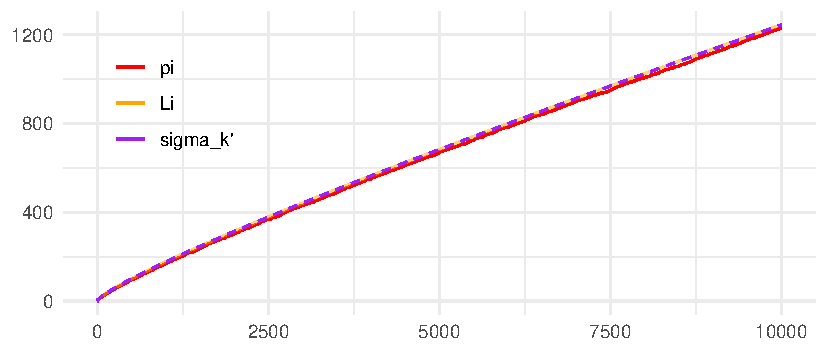
\includegraphics[width=\textwidth,height=6cm]{comparison_odd_prob}
\caption{Graphes des fonctions $\pi$ et $\sigma$.}
\label{fig:comparison_sigma_prob}
\end{figure}

\begin{figure}[H]
	\centering
	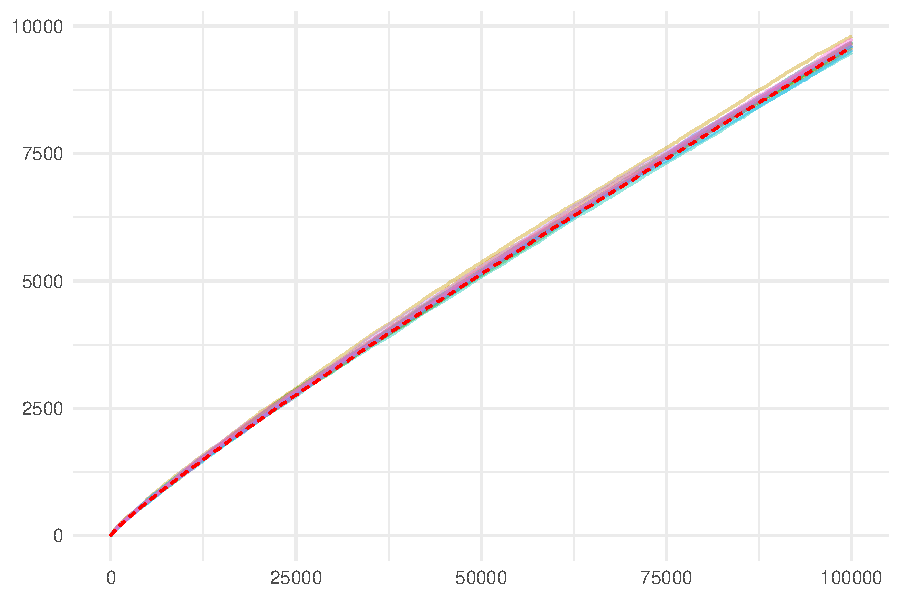
\includegraphics[width=\textwidth]{prob_sample_odd}
	\caption{graphes des fonctions $\sigma_k$ pour $k \leq 25$ (25 premiers ensembles impairs) et $\pi$}
	\label{fig:prob_sample_odd}
\end{figure}

\end{document}